\documentclass[buriama8_dp.tex]{subfiles}
\begin{document}

\chapter{Implementation}

We divide the environment into a grid \(10 \times 10 \times 6\) (width \(\times\) height \(\times\) depth, from the viewpoint of the robot. A cell of the grid is a cube with its side 10\,cm long; the whole grid is positioned in front of the robot and is centered horizontally, the lowest cells are 10\,cm above the robot base and the first layer of the grid is 0.5\,m far from the base. To allow the robot to perform any moves at all, we assume that all space between the robot and the explored space, including the space behind the robot, is known, which is a reasonable assumption, since the mobile robot supposedly came from there and knows the environment. We further assume a static environment is to be explored.

The robot will move the sensing tool through the grid, following a CPP algorithm. The algorithm aims to minimize the path length in the Cartesian space. Once contact with obstacle is detected by the instrument, the motion will stop, the obstacle is registered in both the mapping algorithm and in the robot driver as a confirmed obstacle. The robot then recovers from the touch and proceeds with the exploration. The robot will always avoid colliding the arm with known obstacles, including the mobile robot it is mounted on. It will also avoid reaching into the unexplored space by other parts than the sensing tool. The sensing tool needs to be included in the collision checking model to avoid obstacles and only allowed to enter the space it is to explore.

Making the arm move proved more difficult than expected, with motion planning in tight spaces failing frequently. We managed to offload the motion control to the Jacobian controller, but the planned motion is still unstable and sometimes reports perfectly reachable cells as unreachable.

\section{System architecture}
\label{sec:impl_arch}

The architecture of the system is designed to fit into the modular ROS framework. Each functional part is implemented as a standalone ROS node, which can be used independently on the rest of them. The architecture is illustrated in Figure~\ref{fig:arch}.

\begin{figure}[ht]
  \centering
  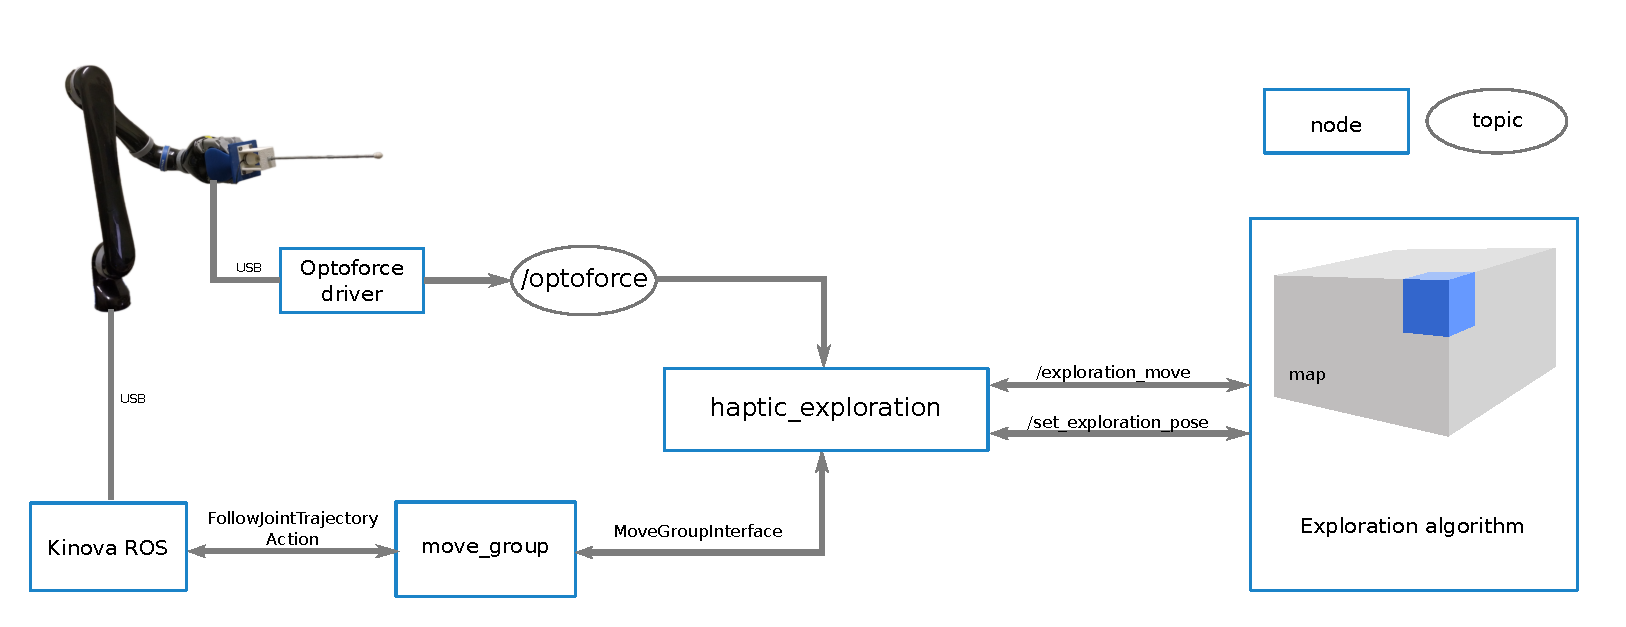
\includegraphics[width=\textwidth]{architecture.pdf}
  \caption{Overview of the system architecture}
  \label{fig:arch}
\end{figure}

A node runs the optoforce driver and publishes the force readings to a common topic. If any other component wishes to use them, they are available system-wide.

The interaction with the robot and the MoveIt-maintained planning scene is done through \code{haptic_exploration} node. The node exposes services that control the robot motion and maintains the state of the arm in the exploration grid. The node runs in one process that listens for exploration requests and carries out the desired motions, while simultaneously processing the data from the Optoforce sensor. As the node needs to process the incoming messages, execute services and publish robot instructions simultaneously, the node event loop is carried out by a \code{AsyncSpinner}, which starts several event-processing threads. The concurrency is automatic, but care needs to be taken when processing the event callbacks in different threads to prevent synchronization issues. The node depends on the \code{move_group} node running with all its configuration loaded, and on the Kinova ROS driver node.

The exploration algorithm runs in an independent process. It communicates with the main node by calling its services for arm movement, and is informed about the results in the service return messages. In this program, the map of the environment is constructed, and, based on it, the appropriate movements are sent to the main node.

\section{Optoforce driver}
\label{sec:opto_driver}

The Optoforce driver node is implemented in Python. Our implementation is based on an open-source driver \cite{opto_driver}.

The driver connects to the emulated serial port on the system, which requires the user to have sufficient privileges to do so. The sensor is first configured to send the measurements at 100\,Hz, together with parameters of the data pre-processing done in the DAQ unit, like filtering.

The driver then starts receiving measurements over the serial line, which are decoded, scaled to Newtons by the calibrated sensitivity scale provided by the manufacturer. Then, the values are published as a \code{Vector3} message to the \code{\optoforce} topic.

\section{Robot motion}
\label{sec:rob_impl}

We mentioned two different ways of driving the arm in Section~\ref{sec:moveit}. As both have their pros and cons, we implemented both of them and tested them to decide which one to use. The experiment testing the implementation is described in Section~\ref{subsec:exp_move_real}.

The control code is implemented in C++ to ensure optimal performance in the critical control code, as well as to leverage the more feature-rich API MoveIt exposes through the C++ module \code{MoveGroupInterface}. A python interface exists as well, but has limited capabilities.

Collision checking is performed to prevent arm and tool damage. The unknown space is filled with collision cubes, one for each grid cell. This ensures the arm stays safe. The tool is represented by a collision cylinder the size of the stick attached to the end effector. All collision checks in both motion control methods include the tool so that it does not get damaged. Only when a cell is to be explored, its collision cube is removed to allow the stick to enter it and explore it. A better way to implement it would be to modify the allowed collision matrix to allow collisions only between the stick and the cube, instead of anything and the cube as it is now. MoveIt however suffers heavily from synchronization issues, as the structures live in both the \code{move_group} and the user process, and modifying the collision matrix used in planning appears impossible.

The robot control services are implemented in the main node. They can however be easily separated into standalone units, that can be reused in other projects that require driving the arm.

\subsection{Jacobian-driven motion}
\label{subsec:impl_drv_jacob}

As we wrote, for a Cartesian twist (linear and angular velocity) vector \(\vec v\), we can obtain joint velocity \(\dot{\vec q}\) which will result in end effector movement with the given twist. This can be done by calculating the Moore-Penrose pseudoinverse of the Jacobian matrix, preferably through SVD. Details are given in Section~\ref{subsec:no_plan}.

The whole process of obtaining joint velocities for a given twist is already implemented in MoveIt, including Jacobian computation. The method is a part of MoveIt C++ library class \code{RobotState}, which represents the joint configuration of the manipulator. MoveIt expects the twist to be in the end effector reference frame, and thus the Cartesian twist in the world coordinates we use needs to be transformed into that reference frame first. The computation is implemented exactly as stated above, with checks on the singular values during the pseudoinverse computation to guarantee numerical stability of the approach. Near singularities, even the correct results contain very high joint velocities that need to be corrected in order to be executed on the robot, whose joint velocities are limited.

When joint velocity limit of 0.8\,s\(^{-1}\) is violated, we attempt to resolve it by slowing the end effector twist down to 50\% of its original speed. This check is applied until the joint speeds are within limits, or at most 4 times. If the joint speeds are still too high, the motion stops immediately and a failure is reported for the command issuer to do something else.

The complete algorithm is presented in pseudocode as Algorithm~\ref{alg:jacob}.

\begin{algorithm}[htp]
\begin{algorithmic}
  \State \textbf{Input:}
  \State \(\vec v \gets\) Cartesian twist
  \State \(\vec p_t \gets\) target position
  \vspace{1em}

  \While{\(\vec p_t\) is not reached with tolerance \(\epsilon\)}
    \State \(\vec p \gets \) current arm state
    \Comment \parbox[t]{.4\textwidth}{Represents both joint angles and end effector position}
    \State \(\vec e_c \gets \) Cartesian error of \(\vec p\)
    
    \If{\(\vec e_c > \epsilon_{max}\)}
      \State \textbf{return} failure
    \EndIf

    \State \(\vec v_t \gets \vec v + P \vec e_c\)
    \Comment \m P is P-regulator constant

    \State \(\dvec q \gets \)computeJointVelocity(\(\vec p, \vec v_t\))
    \vspace{1em}

    \While{checkVelocityLimit(\(\dvec q\)) fails or at maxiumim 4 times}
      \State \(\vec v_t \gets \frac{1}{2} \vec v_t\)
      \State \(\dot{\vec q} \gets \)computeJointVelocity(\(\vec p, \vec v_t\))
    \EndWhile

    \If{checkVelocityLimit(\(\dvec q\)) fails}
      \State \textbf{return} failure
    \EndIf
    \vspace{1em}

    \State \(\vec p_n \gets \vec p + \dvec q \Delta t\)
    \Comment \parbox[t]{.4\textwidth}{\(\Delta t\) is the duration of one loop, here 20\,ms}

    \If{collisionCheck(\(\vec p_n\)) reports collision}
      \State \textbf{return} failure
    \EndIf
    \vspace{1em}

    \State publishJointVelocityTwice(\(\dvec q\))

    \State run loop at 50\,Hz
    
  \EndWhile
  \State \textbf{return} success
\end{algorithmic}
\caption{Jacobian motion control}
\label{alg:jacob}
\end{algorithm}


The motion is controlled in a control loop running at 50\,Hz. In each iteration, we first compute the twist we need to apply. It consists of a constant input velocity the robot is requested to follow, and a correction term determined by a P regulator that corrects arm deviations from the desired trajectory. Then, MoveIt computes the joint velocities that will result in the computed twist in current arm configuration. The joint velocity checks stated above are then applied, including the eventual update of the twist and joint velocity re-computation.

When the output joint velocities are known, the robot motion with those velocities until the next iteration is simulated. The state expected to be reached by next control loop iteration is checked for collisions, both self- and with the environment. If a collision would occur, the motion is stopped immediately.

When the final joint velocities are computed and verified, they are published to the robot driver topic controlling joint velocities. The same velocities are published twice to match the control loop frequencies (see Section \ref{subsec:api_cart_vel}).

The motion stops when the desired end point is reached. Currently, the robot can be driven through cells of the grid defined by the exploration algorithm, and only move along one axis (to the 6-neighborhood of the current cell) by a given number of cells. The algorithm could easily be extended to follow arbitrary lines. The algorithm also does not try to error correct orientation changes.

The motion is initiated by a calling service \code{/exploration_move}, which is called by message  \code{ExplorationPointRequest} which has three integer parameters \m x, \m y and \m z. They specify the direction and number of cells the robot is to move by. Only one of the numbers can be non-zero, the service call will fail otherwise. The response contains two boolean fields: \code{reached} that indicates if the target cell was reached, and \code{obstacle} that defines whether an obstacle was detected by the sensing tool. If \code{reached} is false, the content of \code{obstacle} is undefined.

\subsection{Planned motion}
\label{subsec:impl_drv_plan}

The planned motion control is implemented using the user-friendly interface of MoveIt, the \code{MoveGroupInterface}. The motion is started by calling service \code{/set_exploration_pose}. The request is, as with Jacobian control, an \code{ExplorePointRequest} with \m x, \m y and \m z fields. Here, the fields specify the point in the grid that is to be explored by planning a path that reaches it. The output is the same as in Jacobian control.

When the request is received, the target pose is specified to MoveIt, collisions of the sick and the target cell's cube are allowed and a motion plan is computed. We use the LBKPIECE motion planner provided in MoveIt. If the planning is unsuccessful, it is retried at most two times (plans may fail to be found in close proximity to obstacles for example). If no solution is found then, an unreachable cell is reported to the exploration algorithm by returning \code{reached} as false.

Once the plan is computed, movement is initiated through the \code{MoveGroupInterface} and the node waits for its completion. If the execution was successful, the exploration can proceed and a free cell is reported. If an obstacle was detected during the motion (see Section~\ref{subsec:impl_stop}), the fact is propagated to the caller and the movement stops immediately.

\subsection{Hybrid solution}
\label{subsec:impl_drv}

\hyphenation{Move-Group-Interface}

The algorithms we use employ both transitions to a neighboring cell and long moves to distant cells. To implement short transitions, we use the Jacobian control in conjunction with the planning as fallback.

We first try to complete the movement by Jacobian control. If the movement fails, either because it encountered a singular configuration of the arm, because the arm would collide with an obstacle or because joint limits, both angular and velocity) would be violated, the algorithm returns back and tries to reach that cell again by planning the motion, possibly several times. Note that on contact detection by the instrument the movement is stopped as well, but it is a success.

When exploring the cells in the lower part of the arm workspace, it is beneficial to orient the sensing tool downward. The reasons are twofold: one, the wrist rotation with respect to the 3rd arm link is limited, and pointing the instrument forward could be infeasible, and two, the instrument can then sense the ground below the robot without crashing into it first. The orientation change cannot be handled by the Jacobian controller because such control was not implemented. We instead plan the motion, also using the plan that reaches an exact location to correct any errors that would have accumulated during driving the arm by the Jacobian controller.

\subsection{Stopping the movement}
\label{subsec:impl_stop}

The main node is subscribed to the force readings published by the Optoforce sensor. The messages are processed asynchronously to all other operation by the \code{AsyncSpinner}.

The force readings are checked against the thresholds of 2\,N for lateral and 4\,N for axial forces. If the thresholds are exceeded, the node enters stop state and all motion is stopped. If there is a plan execution currently in progress, it is stopped via the \code{MoveGroupInterface}. The Jacobian-controlled movement is stopped in the control loop if the node is in stop state.

If the motion was planned, the arm traces its steps back by following the motion plan backwards until the tool leaves the newly classified obstacle. Then, the exploration algorithm can determine the next cell to be explored and request a planned motion to it (Cartesian control cannot be used, as we are not in a grid cell when we have left the obstacle).

When the motion is stopped during Jacobian controlled motion, the robot then reverses the motion and returns back where it came from. As the robot was there previously, the movement is necessarily safe. Nonetheless, all the collisions are still checked.

Once the contact between the tool and the obstacle ceases and the forces drop below the thresholds, the main node returns to normal state. We use the same thresholds here instead of lower values causing hysteresis because we do not base any action on the force drop, we only continue in the retracting movement.


\section{Exploration algorithm}
\label{sec:alg_impl}

We implemented both the CPP algorithms we mentioned as feasible in Section~\ref{sec:cpp_comp}, the compact space heuristic and the neural-network (NN) algorithm. Only the heuristic algorithm is adapter to drive the arm; the neural-network algorithm did not show promising results in the simulated test \ref{sec:exp_sim_coverage}. The algorithms are implemented in python and are at the moment run as commands by the user. They can easily be transformed into actions or services that are called by other components of the system.

Both the algorithms share the same basic structure. The map is represented in a 3D integer array. The arm workspace is specified to the algorithms by marking the unreachable fields as obstacles before the algorithm starts. All other cells are set to the base value of 0. The environment is searched layer by layer; in the \m y direction in our case.

\subsection{Heuristic algorithm}
\label{subsec:impl_heur}

In each layer, the heuristic algorithm explores all the cells sequentially. The current cell is marked in the map as empty, as obstacle or as unreachable based on the outcome of the effort to reach the cell. The information about the current cell is propagated to the neighboring cells, adding 1 if the current cell is empty and 2 if it is an obstacle. This way, each yet unexplored map cell holds the value of the heuristic function defined in Equation~\ref{eq:heuristic}. Then, the next cell is found by simply choosing the neighbor with the highest heuristic value and breaking the eventual ties as defined in \ref{sec:my_heuristic}.

If no neighboring cell is unexplored, the nearest such cell is found and set as the next exploration target. If no such cell exists, the robot moves the the nearest free cell in the following layer.

\subsection{Neural-network-inspired algorithm}
\label{subsec:impl_neuro}

The NN needs, beside the map, another two arrays that represents the activity of the neurons in the network and their external inputs. Only one map layer needs to be simulated at a time, so 2D arrays are in order. The activity array is initialized to zeros, while the external inputs are initialized to the corresponding map layer. The parameters of the method are set according to the original article \cite{neural}: \(A=50, B=2, D=1, E=100\).

We made a few changes to the algorithm. First, we do not take direction changes of the robot into account as does the original algorithm. The article fails to specify the weight with which the turning angle is to be added to the activity anyway. Second, when all the neighboring cells are either already explored or obstacles, we move the robot to the closest unexplored cell as in our heuristic algorithm. The original is meant to be used with whole robots in planar environment, and as such could not move the robots around at will as we can the robotic arm.

The neural network is modeled by differential Equation \ref{eqn:shunting}. As we decide to move the robot based on the activity, we need to model the behavior of the network in time to simulate the activity propagation and compute the appropriate values for neuron activity. We simulate the activity function by the Runge-Kutta 4th order method, which has a great ratio between performance (high precision) and implementation complexity (low).

We simulate the network in 0.05\,s steps. In the beginning of each layer, we run the simulation for 100 steps to let the activities stabilize. Then in each step, the robot chooses the neighboring cell with highest activity. If all neighbours are have lower activity than the current cell, and are thus already explored or obstacles, we move the robot to the nearest unexplored cell. If there is no such cell left in this layer, the robot moves to the following layer.

\section{Integration with the Absolem robotic platform}
\label{sec:integr}

The software implemented in this thesis is designed to be integrated into the TRADR project, to use the arm when mounted on the mobile robot platform and explore space as needed by the whole robot's goal. The main concern with the integration is obstacle avoidance for the arm, wchich needs to take the platform itself into account. That should not pose a problem, as complete collsion checking is performed even now, and it is only a matter of adding the platform collision model into the environment.

The second matter is the interface via which the whole exploration will be invoked. This will need to be agreed upon by the designers of the components that are to be the initiators of the exploration, including the map format to be returned; if it is to be a point cloud, a representation of the grid or something completely different. 

\end{document}


%%% Local Variables:
%%% mode: latex
%%% TeX-master: "buriama8_dp"
%%% End:
